%---------------------
\pagestyle{plain}
\setcounter{page}{1}
\pagenumbering{arabic}
%---------------------

\chapter{مقدمه}


محوریت کار ما قرار است\cite{calcul} باشد که در آن سعی شده روش وارسی مدل با کمک نظریه تعبیر مجرد، بهبود داده شود. در\cite{clarke} روشی که معرفی شده در‌واقع ویژگی برنامه‌ها را به کمک منطق های \lr{LTL} یا \lr{CTL} بیان می‌کند. خود برنامه‌ها هم با کمک معناشناسی این منطق ها که نوع خاصی از مدل های کریپیکی به اسم سیستم گذار هستند توصیف می شوند. اما در\cite{calcul} کاری که انجام شده به این شکل است که منطق های \lr{LTL} و \lr{CTL} با عبارات منظم\cite{kleene56} جایگزین شده‌اند. علت این کار دو نکته بوده، اولی اینکه استفاده از عبارات منظم به جای منطق های نام برده شده می‌تواند برای برنامه نویسان ساده‌تر باشد و دومی اینکه عبارت منظم از از منطق های نام برده شده قدرت بیان بالاتری دارد.\cite{regisbetter} در ادامه ی کار وارسی مدل با استفاده از موجودات جدید تعریف شده به سه شکل مختلف بیان شده. در هر مرتبه بیان وارسی مدل، به‌گفته‌ی نویسنده، "ساختارمند"تر شده. می‌توان دریافت که فایده ساختارمندتر بودن بیان این است که پیاده‌سازی راحت‌تری دارد.\\
حال به بیان و بررسی تعاریف و خواص آن‌ها می‌پردازیم.


\section{روش وارسی مدل}

روش وارسی مدل یک روش صوری است که برای درستی‌یابی سیستم‌های مختلف استفاده می‌شود. در این روش معمولا ابتدا یک ماشین حالات متناهی از روی سیستم مورد بررسی ساخته می‌شود، سپس بررسی‌هایی که قرار است روی سیستم اصلی انجام شوند، روی این ماشین( مدل) انجام می‌شود. در بررسی صحت کارکرد برنامه‌های کامپیوتری از این روش استفاده می‌شود اما این تنها مورد استفاده از این روش نیست و هر منظومه‌ی دیگری که قابلیت بیان به صورت صوری را داشته باشد قابل بررسی با این روش هست. مثلا می‌توان از این روش برای بررسی صحت عملکرد برنامه‌ی قطارهای شهری استفاده کرد; در حالتی که مثلا خصوصیات مورد بررسی ما عدم رخ دادن تصادف بین قطارها یا پوشش تمام  مناطق شهر باشد. مثال های دیگر استفاده‌ی این روش در علوم کامپیوتر می تواند بررسی صحت عملکرد یک پردازنده یا مثلا الگوریتم تقسیمِ وظایف یک سیستم عامل باشد. این مثال‌ها هیچ یک برنامه‌ی کامپیوتری نیستند( هر چند که ممکن است مجبور باشیم از یک برنامه‌ی کامپیوتری برای پیاده سازی آن‌ها کمک بگیریم که در آن صورت بررسی صحت عملکرد آن برنامه‌ی کامپیوتری داستانی دیگر خواهد داشت) اما قابل بیان به صورت صوری به جای زبان طبیعی هستند.

ایده‌ی روش وارسی مدل از منطق‌های زمانی مختلف استفاده می‌کند. منطق زمانی یک نوع منطق موجهات است. منطق‌های موجهات از گسترش زبان منطق کلاسیک با اضافه کردن ادات وجهی گوناگون، با معانی متفاوتی که ممکن است در زبان طبیعی داشته باشند، ساخته می‌شوند. این ادوات غالبا در زبان طبیعی نقش قید را دارند. منطق‌های زمانی بخشی از منطق‌های موجهات هستند که به صوری‌گری ما مفهوم زمان را هم اضافه می‌کنند، یعنی قیدهایی مانند فعلا، بعدا و قبلا. منطقی که در اینجا بیان می‌کنیم \lr{LTL} نام دارد که یکی از منطق‌های زمانی است که برای روش وارسی مدل استفاده می‌شود. البته در مورد قیدهایی که نام بردیم ذکر این نکته ضروری است که در این بیانی که ما در اینجا از این منطق ارائه داده‌ایم ادوات جدید این فعل‌ها نیستند، هرچند که به کمک ادوات جدید می‌توان ادواتی برای هر یک از این قیود ساخت.
این تکه از \cite{buchi} آورده شده.

ابتدا زبان این منطق را بیان می‌کنیم و سعی می‌کنیم به طور غیر دقیق در مورد معنای فرمول‌های این زبان به خواننده یک درک شهودی بدهیم; سپس به سراغ معناشناسی صوری این منطق می‌رویم.

\subsection{زبان \lr{LTL}}
\begin{defn}
	هر عضو مجموعه‌ی $\Phi$ یک فرمول در زبان \lr{LTL} است( و $\Pi$ مجموعه‌ی فرمول‌های اتمی است و $\pi \in \Pi$):
	$$
	\Pi \subset \Phi,
	$$
	$$
	\phi \in \Phi \Leftrightarrow
	\phi ::= \pi | \phi \lor \phi |
	\neg \phi |
	\bigcirc \phi |
	\phi \mathcal{U}\phi 
$$	
	
\end{defn}
اولین نکته‌ای که برای فرمول‌های این زبان به آن نیاز داریم این است که در این منطق ما زمان را با اعداد طبیعی و هر خاصیتی که در موردشان تعریف شده نشان می‌دهیم. یعنی برای یک فرمول، زمان از عدد ۰ شروع شده و تا ابد ادامه خواهد داشت و حین گذر زمان ممکن است ارزش فرمول‌ها تغییر کند. مسلما پس از بررسی معناشناسی صوری بهتر می‌شود این مفهوم را به طور شهودی حس کرد، اما به هر حال به خواننده پیشنهاد می‌شود پیش از رسیدن به آن بخش به ادامه‌ی این بخش هم توجه شود. 

در این زبان ادوات کلاسیک 
$\neg, \lor$
هستند با همان معنایی که در منطق گزاره‌ای کلاسیک داشتند.  
در ادوات جدید 
$\bigcirc \phi$
به معنای برقرار بودن این فرمول دقیقا در لحظه‌ی بعدی( دقیقا یک لحظه) است، مثلا در شکل زیر با در نظر گرفتن اینکه در زمان 0 هستیم، این فرمول در لحظه‌ی ۱ برقرار است.
	\begin{center}
	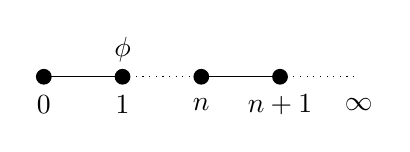
\begin{tikzpicture}
	\node at (1,0.35) (phi) {$\phi$};
	\node at (1,-0.35) (1) {$1$};
	\node at (0,-0.35) (0) {$0$};
	\node at (2,-0.35) (n) {$n$};
	\node at (3,-0.35) (1) {$n+1$};
	\node at (4,-0.35) (1) {$\infty$};
	\fill (0,0) circle (0.1cm);
	\fill (1,0) circle (0.1cm);
	\fill (2,0) circle (0.1cm);
	\fill (3,0) circle (0.1cm);
	\path (0,0) edge (1,0) 
	(1,0) edge[dotted] (2,0)
	(2,0) edge (3,0)
	(3,0) edge[dotted] (4,0);
	\end{tikzpicture}
\end{center}
$\phi \mathcal{U}\psi$
به این معنی است که فرمول سمت چپی حداقل تا قبل از اینکه فرمول سمت راستی برقرار شود، برقرار است.( مثلا اگر بگوییم "تا وقتی که باران نباریده زمین خشک است" در این صورت "زمین خشک است" به جای فرمول سمت چپ و "باران باریده است" فرمول سمت راست است).
\begin{center}
	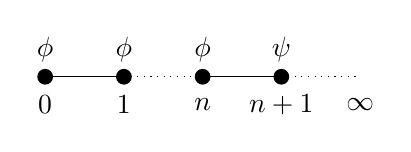
\begin{tikzpicture}
	\node at (1,0.35) (phi) {$\phi$};
	\node at (0,0.35) (phi) {$\phi$};
	\node at (2,0.35) (phi) {$\phi$};
	\node at (3,0.35) (phi) {$\psi$};
	\node at (1,-0.35) (1) {$1$};
	\node at (0,-0.35) (0) {$0$};
	\node at (2,-0.35) (n) {$n$};
	\node at (3,-0.35) (1) {$n+1$};
	\node at (4,-0.35) (1) {$\infty$};
	\fill (0,0) circle (0.1cm);
	\fill (1,0) circle (0.1cm);
	\fill (2,0) circle (0.1cm);
	\fill (3,0) circle (0.1cm);
	\path (0,0) edge (1,0) 
	(1,0) edge[dotted] (2,0)
	(2,0) edge (3,0)
	(3,0) edge[dotted] (4,0);
	\end{tikzpicture}
\end{center}

برای این زبان همان‌طور که در منطق کلاسیک از ادوات عطف و شرطی با اینکه با ادواتی که داریم قابل بیان هستند استفاده می‌کنند، ادات بیشتری هم هستند که مورد استفاده قرار می‌گیرند و با همین دو اداتی که معرفی کردیم قابل بیان هستند اما ما در اینجا از آن‌ها اسمی نیاورده‌ایم. دلیل وجود این‌ها هم راحت‌تر کردن کار کسی است که قرار است یک خاصیت را به صورت یک فرمول در این زبان بیان کند. همان طور که استفاده نکردن از یا و شرطی در منطق گزاره‌ای می‌تواند به سخت کردن بیان جملات در چارچوب این منطق منجر شود، حذف این ادوات وجهی هم بیان خواص را در این منطق مشکل می‌سازد. اما از آنجاییکه ما صرفا این بخش را برای معرفی این ایده قرار داده‌ایم، دیگر به بیان ادات وجهی دیگر نپرداخته‌ایم.

حال که به درکی شهودی از معنای فرمول‌های این زبان رسیده‌ایم، به بیان صوری این مفاهیم می‌پردازیم.

\subsection{معناشناسی \lr{LTL}}

مدل‌های این منطق را به صورت توابع
$M:\mathbb{N}_0 \rightarrow \mathit{P}(\Pi)$ 
تعریف می‌کنیم. یعنی هر مدل یک تابع است که هر عدد طبیعی را به یک مجموعه از فرمول‌های اتمی می‌برد. این در واقع قرار است به این معنی باشد که یک مدل به تعبیری به این معنی است که در هر لحظه کدام یک از فرمول‌های اتمی درست هستند. مثلا در مدلی به نام $M_i$ در واقع
$M_i(5)$
مجموعه‌ی اتم‌هایی است که در لحظه‌ی 5 طبق این مدل درست هستند و اگر اتمی در این مجموعه نباشد ارزش غلط دارد.
درستی یک فرمول در یک مدل را با 
$M,i$
نشان می‌دهیم و 
$M,i \models \phi$
به این معنی است که در لحظه‌ی $i$در مدل $\phi$ ارزش درست دارد. این مفهوم را به صورت بازگشتی به شکل زیر تعریف می‌کنیم:


\begin{flushleft}
$	M,i \models \pi \:\:\: \mathit{iff} \:\:\: \pi \in M(i)$\\
$	M,i \models \neg \phi \:\:\: \mathit{iff} \:\:\: M,i\nvDash \phi$\\
$	M,i \models \phi \lor \psi \:\:\: \mathit{iff} \:\:\: M,i \models \phi \:\:\: \mathit{or} \:\:\: M,i \models \psi$\\
	 $M,i \models \bigcirc \phi  \:\:\:  \mathit{iff} \:\:\: M,i+1 \models \phi$\\
	 $M,i \models \phi \mathcal{U} \psi \:\:\: \mathit{iff} \:\:\: 
	 \exists k \geq i \in \mathbb{N}_0: \forall i\leq j< k: M,j \models \phi \:\:\: \mathit{and} \:\:\: M,k \models \psi$
\end{flushleft}

برای یک فرمول اگر مدلی وجود داشته باشد که در آن مدل آن فرمول صادق باشد، آنگاه آن فرمول را \emph{ارضاپذیر} می‌گوییم. اگر یک فرمول در هر مدلی صادق باشد، آن فرمول را \emph{معتبر} می‌گوییم.\\
شیوه‌ی دیگری برای بیان همین معناشناسی که گفتیم به شکل اتوماتا است. 


\section{نظریه تعبیر مجرد}


